The physical scattering process which gives rise to speckle in the cone is
perhaps best understood in context of \Figure{fig:plasmongeosimple}.  This
simplified scattering model is of course a simplification of the actual system
physics, but as will be shown is a good approximation which captures much of
the observed behavior.

The process is thought of as follows: SPPs are excited and come into existence
at their creation point within the elliptical spot of the evanescent wave
created by the incident beam (in the $x$-$z$ plane).  Once created, an SPP
will propagate, potentially out of the illuminated region, until either
decaying as heat or as a photon scattered into the cone.  The maximum
propagation distance is set as per \Section{sec:sppphysicalchar}.  Since SPPs
which decay as heat are not observed in this experiment, they are neglected.
During propagation, the SPP follows a scattering path, accumulating phase by
visiting one or more scatterers (in-plane scattering).  The ultimate scatterer
is responsible for the SPP decaying as a photon and scattering into the cone
(out of plane scattering).  The superposition of all SPP scattering paths is
responsible for the observed speckle in the cone.

Restated, the individual components of this scattering model are:
\begin{itemize}
\item An elliptical \textit{illuminated region}, representing the incident
				evanescent field used to excite SPPs.
\item \textit{Scatterers}, fixed point defects, typically randomly
				distributed, which can modify the in-plane momentum of an SPP and
				optionally cause it to decay as a photon out of plane into the cone. 
\item A \textit{scattering path}, the ordered sequence of
				scatterers an SPP visits before exiting the system.  
\item An SPP \textit{creation point}, where an SPP comes into existence and
				begins accumulating phase.
\end{itemize}
\begin{figure}[ht]
\centering
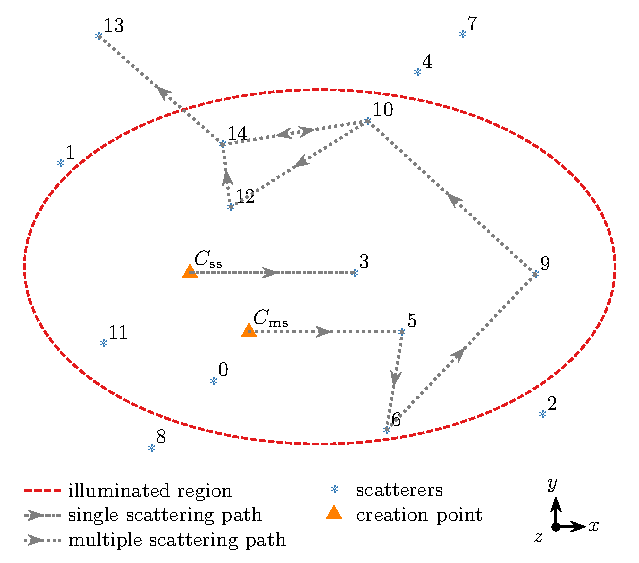
\includegraphics[keepaspectratio]{scatteringmicro/figures/montecarlogeosimple.pdf}
\caption{A simplified SPP scattering model.  An SPP is excited within the
				illuminated region at its creation point and follows a scattering path
				amongst fixed point scatterers.  The scattering path can include one
				(single scattering) or more (multiple scattering) scatterers.
}
\label{fig:plasmongeosimple}
\end{figure}

Physically there are two possible in-plane scattering processes as depicted in
\Figure{fig:scattsinglevmultiple}.  The first is \textit{single scattering},
whereby only one scatterer is visited in each path from source to
observation.  An example single scattering path is depicted in
\Figure{fig:scattsinglevmultiple} by the path $\{C_\mathrm{ss},3\}$: an SPP is
created at $C_\mathrm{ss}$, propagates to $3$, then decays as a photon.

In addition to single scattering, there exists a much more interesting and
phenomenologically complex process known as \textit{multiple scattering}.  In
multiple scattering, each path from source to observation contains multiple
scattering events.  An example multiple scattering path is shown
in \Figure{fig:scattsinglevmultiple} by the path
$\{C_\mathrm{ms},5,6,9,10,12,14,10,14,13\}$.  This example path illustrates
several important assumptions about the behavior of a multiple scattering
path:
\begin{itemize}
\item The same scatterer has the possibility of being visited an arbitrary
				number of times, e.g.\ $\{10,12,14,10,14\}$.
\item Closed loop and time reversed paths are possible, e.g.\ $\{10,12,14\}$.
				In these cases the accumulated phase is the same regardless of
				direction, e.g. $\{10,12,14\} \equiv \{14,12,10\}$.
\end{itemize}

Note the first scatterer visited in both example paths for single and multiple
scattering, $3$ and $5$, are directly downstream of their SPP creation points.
That is to say to a good approximation the first scatterer is always located
in the $+x$ direction; in the coordinate system of
\Figure{fig:plasmongeosimple}, an SPP at its creation point has momentum in
the positive $x$ direction.  Including this assumption in the scattering model
implies that not all scatterers can be reached in a single scattering process
or as the first scatterer of a multiple scattering one, for example
scatterers 1, 13, 8, 4, and 7 in \Figure{fig:plasmongeosimple}.

\subsection{Phase Accumulation and Extension to the Far Field} 
The local in-plane scattering process in the simplified model of
\Figure{fig:plasmongeosimple} will now be extended to model light in the cone.
In \Figure{fig:plasmongeosimple}, each scatterer has a location given by the
Cartesian coordinates $(x,y,z=0)$, where the central point of the prism's
hypotenuse on the far surface of the metal film is the origin $(0,0,0)$.  The
central point of the focus of the incident Gaussian excitation beam (the
illuminated region) is also coincident at $(0,0,0)$.

In the cone, the detector (a two dimensional image sensor) is assigned the
coordinates $(x^\prime,y^\prime,z^\prime)$.  Again, the metal film is in the
$x$-$y$ plane and the incident light in the $x$-$z$ plane.

The field on the detector has either two or three two phase contributions
depending on the scattering order. The first, $\varphi_\mathrm{loc}$, comes
from the phase of the local SPP field propagating on the metal surface in the
$+x$ direction to the first scatterer,
\begin{equation}
\varphi_\mathrm{loc} = \ksp x.
\label{eqn:smicrofirstphase}
\end{equation}
In the example paths of \Figure{fig:plasmongeosimple}, $x$ in
\Equation{eqn:smicrofirstphase} would be the $x$
coordinate of either scatterer $3$ or $5$.  Given an SPP is in phase with the
exciting field, the choice of the origin and this first phase is arbitrary,
but is expressed as given in \Equation{eqn:smicrofirstphase} for simplicity.

The second phase contribution, $\varphi_\mathrm{ff}$, is phase accumulated
from the final out of plane scatterer to the detector in the far field,
\begin{equation}
\varphi_\mathrm{ff} =
k_0\sqrt{{(x-x^\prime)}^2+{(y-y^\prime)}^2+{(z-z^\prime)}^2},
\label{eqn:smicrosecondphase}
\end{equation}
where $x$, $y$, and $z$ would assume the coordinates of the final scatterer,
$3$ or $13$ in the example paths of \Figure{fig:plasmongeosimple}.

Given Equations~\ref{eqn:smicrofirstphase} and~\ref{eqn:smicrosecondphase},
the field on the detector for an individual path in the case of single scattering is given by
\begin{align}
\mathbf{E}(x^\prime,y^\prime,z^\prime) &=
\mathbf{E}_0\exp\bigl(\mi(\varphi_\mathrm{loc}+\varphi_\mathrm{ff})\bigr)\\
&= \mathbf{E}_0\exp\!\left(\mi\ksp x + %
\mi k_0\sqrt{{(x-x^\prime)}^2+{(y-y^\prime)}^2+{(z-z^\prime)}^2}\right).
\label{eqn:smicrosinglescattering}
\end{align}
Or in spherical coordinates with the detector at
$(\rho^\prime,\theta^\prime,\phi^\prime)$,
\begin{align}
				\mathbf{E}(\rho^\prime,\theta^\prime,\phi^\prime) &= \mathbf{E}_0\exp\Bigl(\mi\ksp x \\
&+ \mi k_0\sqrt{{(\rho^\prime\sin\theta^\prime\cos\phi^\prime
x+x)}^2+{(\rho^\prime\sin\theta^\prime\sin\phi^\prime+y)}^2+{(\rho^\prime\cos\theta^\prime+z)}^2
} \Bigr).
\label{eqn:scattspherical}
\end{align}
Again, $x$, $y$, and $z$ are the coordinates of the sole scatterer in an
individual path of the single scattering process.  Furthermore, note that the
refractive index change from prism to air has been neglected.  To a good
approximation, the hemispherical geometry imparts only a constant phase to the
sum, and therefore has no observable effect on the speckle pattern.

For a system with $M$ total scatterers and $N \leq M$ scatterers downstream of
a creation point within the illuminated spot, the single scattering process
has $N$ unique phasors for each $N$ paths.  The $n$th path then has a phase
$\varphi_n = \varphi_\mathrm{n,loc}+\varphi_\mathrm{n,ff}$.  Assuming each
scatterer is visited with equal probability and SPPs re-radiating as photons
are scattered isotropically into the cone, the field on the
detector is given by the coherent superposition of the paths,
\begin{equation}
\mathbf{E}(x^\prime,y^\prime,z^\prime) =
\sum_{n=0}^{N-1}
\mathbf{E}_n \me^{\mi{(\varphi_\mathrm{n,loc}+\varphi_\mathrm{n,ff})}},
\end{equation}
where $\mathbf{E}_n$ is the fractional contribution of each scattering path to
the total amplitude of the electric field $\mathbf{E}_0$ set by the incident
beam
\begin{equation}
\sum_{n=0}^{N-1}\mathbf{E}_n = \mathbf{E}_0.
\end{equation}

For a multiple scattering process, a third phase term,
$\varphi_\mathrm{ms,n}$, must be included for each scattering path.
$\varphi_\mathrm{ms,n}$ accounts for in-plane multiple scattering, where each
of $N$ total paths visits $K$ scatterers amongst the $M$ total.  If the
ordered scattering sequence for the $n$th path is given by $S_{n,0} \ldots
S_{n,{K-1}}$, and the positions of the $k$th scatterer in the path sequence
$(x_{S_{n,k}},y_{S_{n,k}},z=0)$, the phase accumulated for the $n$th path from
multiple scattering is
\begin{equation}
\varphi_\mathrm{ms,n}=\sum_{k=0}^{K-2}
\sqrt{{(x_{S_{n,{k+1}}}-x_{S_{n,k}})}^2+{(y_{S_{n,{k+1}}}-y_{S_{n,k}})}^2}.
\end{equation}
The length of $S_n$ and its ordered sequence is produced by a stochastic
process and will vary from path to path.  The field on the detector
for multiple scattering is then given by the superposition of all paths from
creation to detector
\begin{equation}
\mathbf{E}(x^\prime,y^\prime,z^\prime) =
\lim_{N\to\infty}
\sum_{n=0}^{N-1}
\mathbf{E}_n
\exp\!\big({\mi{(\varphi_\mathrm{n,loc}+\varphi_\mathrm{n,ff}+\varphi_\mathrm{n,ms})}}\big).
\label{eqn:smicromsphase}
\end{equation}

\Equation{eqn:smicromsphase} is akin to the path integral formulation of
quantum mechanics.  By letting $N\to\infty$, all possible sequences of $S_n$
(again, produced by a yet unspecified stochastic process) will be explored by
the multiple scattering paths weighted by $\mathbf{E}_n$.  In the present set
of experiments with a \SI{50}{\milli\watt} diode laser, the limit in
\Equation{eqn:smicromsphase} is for all practical purposes fulfilled.
Furthermore it will be assumed that the number of scatterers $M$ is sufficient
to produce speckle with statistics given by the random phasor sum model
(\Equation{eqn:phasorsum}).

\subsection{Transition from Single to Multiple Scattering}
The transition from the single to the multiple scattering occurs roughly upon
fulfillment of the Ioffe-Regel criterion~\cite{ioffe1960non}, when the
transport mean free path $l^*$ is much larger than the spatial frequency of
the optical wave, or
\begin{equation}
k l^* \approx 1
\end{equation}
where $k=\omega/c$ as usual.  The transport mean path is defined as the
characteristic distance over which the incident wave is scattered out of its
incoming direction~\cite{berkovits1994correlations}.  This is the optical
analog of electron transport in condensed matter physics.  There, one would
use the Fermi wavenumber $k_F$ and take $l^*$ to be the mean free path.
Materials for which $k_F l^* \gg 1$ are conductors, and materials for which
$k_F l^* \ll 1$ are insulators.  The multiple scattering regime can also be
defined in terms of the sample length $L$, such that if $l^* \ll L$ and $1/(k
l^*) \ll 1$, the system can be thought to be the multiple scattering regime.

Xxxxxxxxxx is the cone really isotropic?  show a picture xxxxxxxxxxx

%If the detector is in the far field, $\rho^\prime\gg\lambda_0$,
%\Equation{eqn:scattspherical} can be simplified.  First the additional optical
%path length accumulated propagating through the prism is neglected.  Second,
%if the path length \textit{difference} between the origin and the far field is
%used, \Equation{eqn:dingusthusly} becomes
%\begin{equation}
%\mathbf{E}(\rho^\prime\gg\lambda,\theta^\prime,\phi^\prime) = \exp\!\big( \mi \ksp x
% + \mi k_0 \sin\theta^\prime \left(x\cos\phi^\prime+y\sin\phi^\prime\right)
% + \varphi\big)
%	\label{eqn:primarystripes}
%\end{equation}
%where we have included the variable $\varphi$ to represent the complex phase term
%from non-tip-scattering events (a coherent background).  
